% !TEX root = ../main.tex
\fancychapter{Solution}%
\label{chap:solution}
\cleardoublepage{}

\noindent
Despite strides in enhancing performance and efficiency of geometric constraint
solving approaches, briefly discussed in \Cref{sec:intro.constraints}, the core
issue lies in the generality of geometric constraint solvers.  Although several
approaches employ efficient methods to find a solution, they resort to solving
potentially well-known problems generically when computationally lighter
solutions exist.  Instead of delegating the problem to a solver, a more
efficient approach would be to pinpoint the type of geometric constraint itself,
specializing a solution for several applicable entities.  Take the tangency
constraint as an example: positioning two circles tangent to each other or a
line tangent to an ellipse.  Depending on the inputs, these constraints might
have particularly efficient solutions for each case, in kind making the
computation more efficient.

Classical numerical methods constitute alluring alternatives to the predominant
graph-based approaches.  Having been studied for several decades, even if the
provided solution does not encompass all the possible values within the
problem's domain, they can be used to target specific problems efficiently.
Nonetheless, these suffer from robustness issues discussed in
\cref{sec:related.robustness}, effectively yielding inaccurate solutions if
precautions aren't taken.  A similar argument can be made about algebraic
methods.

This work aims to implement a series of geometric constraint primitives in an
already expressive \ac{TPL} to overcome the need for the specification of
unnecessary details when modeling geometrically constrained entities, promoting
an easier and more efficient usage.  Choosing to implement these in a \ac{TPL}
further avoids the poor scalability with increasing code complexity that arises
from what could be analogous specifications in a \ac{VPL}, a subject previously
discussed in \cref{sec:intro.ad}.

Moreover, by relying on an exact geometry computation library, one of the core
features of this solution lies in the capability of transparently dealing with
plenty of the previously addressed robustness issues.  The user can then resort
to these primitives, and, by composing them, elegantly specify the set of
geometric constraints necessary in order to produce the idealized model.  Since
the available primitives will implement specialized solutions for a finite set
of shapes the user can utilize in whichever combination possible during the
design process, the solution will be exempt of a generic solver component,
potentially boosting performance of design generation.

\Cref{fig:solution.arch} shows the typical \ac{AD} workflow and how the proposed
solution could be integrated with the \ac{AD} tool.  The encapsulated modules in
the figure represent the underlying computation library as an external
component, featuring the geometric constraint primitives library and the code
wrapping the computation library.

\begin{figure}[htb]
  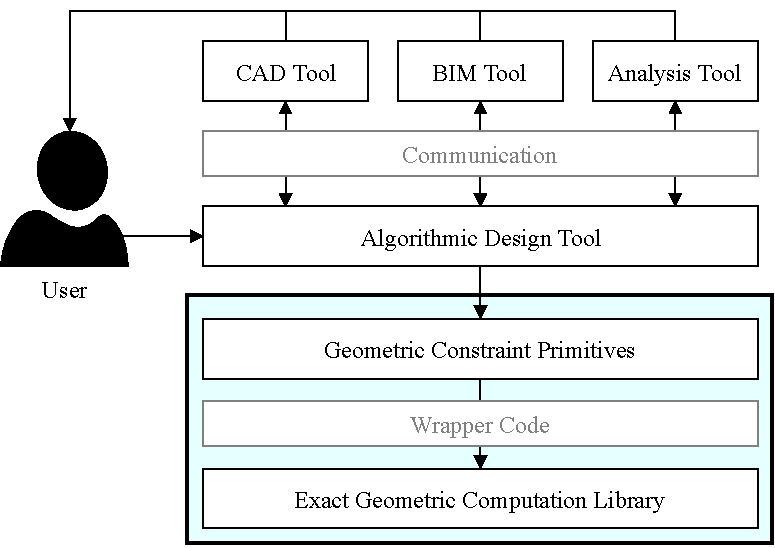
\includegraphics[width=\textwidth]{fig/solution-arch}
  \caption[Solution architecture within AD workflow]{
    General overview of the solution's architecture encapsulated within the
    blue colored box beneath a depiction of the typical \ac{AD} workflow.}%
  \label{fig:solution.arch}
\end{figure}

The following sections go over the components in \cref{fig:solution.arch},
namely the \textit{Exact Computation Geometric Library}, the \textit{Wrapper
Code}, and the \textit{Geometric Constraint Primitives}.  Additionally, we
discuss a few trade-offs from tackling the problem in this fashion as opposed to
potential alternative routes, describing advantages and disadvantages of our
approach.

% !TEX root = ../../main.tex
\section{Implementation}%
\label{sec:solution.impl}

This section details implementation choices with regard to the chosen platforms
for realizing the initially proposed general solution architecture, previously
illustrated in \cref{fig:solution.arch}. Following a brief analysis, we expand
specifically on the concrete components corresponding to the ones within
\cref{fig:solution.arch}'s light blue rectangle.

Examining the \ac{AD} workflow portion of \cref{fig:solution.arch}, there are
depictions of \ac{CAD}, \ac{BIM}, and analysis tools, of which examples could be
Rhinoceros3D, Autodesk's Revit, and Radiance, respectively, with no particular
focus on any of them.  Digging a layer deeper, we find the \ac{AD} tool, which,
by means made available by the tools above it, produces models specific to those
tools from a description provided by the user.  The \ac{AD} tool we have chosen
was
Khepri\footnote{\url{https://github.com/aptmcl/Khepri.jl}}~\cite{Leitao:2019:GRUGEAV},
a text-based tool written in the Julia programming
language~\cite{Bezanson:2017:JAFANC}.  Khepri is the successor of another
text-based \ac{AD} tool named Rosetta~\cite{Leitao:2011:PGDCAD}, a tool written
in the Racket programming language~\cite{PLT:2010:Reference}.  It follows that
the \primitives{} were implemented in the Julia language as well, supported by
an \geomlibrary{}.  The library chosen for the effect was
\ac{CGAL}~\cite{CGAL:5.3:Project}, a highly performant and robust geometric
library written in the C++ programming language~\cite{Stroustrup:2013:CPP}.
\Ac{CGAL} is a comprehensive, mature, open-source library, offering plenty of
data structures and functionality of varying complexity, focusing to provide
easy access to efficient and reliable geometric algorithms.

The language disparity between the \primitives{} module (Julia) and the
\geomlibrary{} (C++) requires a solution for language interoperation.  In other
words, we need to make \ac{CGAL} available to the Julia language.  The Julia
language already possesses facilities that invoke functionality within libraries
written in the C~\cite{Kernighan:1988:C} or the
Fortran~\cite{Backus:1957:Fortran} programming languages, an interfacing
mechanism is commonly known as \ac{FFI}.  It allows for the repurposing of
mature software libraries in foreign languages without the need for a complete
rewrite or adaptation.\footnote{The decision to include such a mechanism at the
language's core by the language designers makes it so that the language can gain
traction early, biding time to later explore native implementations.  Arguably,
it may be one of \textit{the} fundamental features that made the language as
popular as it is and kept it afloat, unlike other similar historical examples
that might have lacked such a mechanism.}  Despite only addressing libraries
written in C and Fortran, this mechanism can also in turn be leveraged and built
upon to interface with other programming languages, e.g., Java, Python, MATLAB,
and, C++.\footnote{There is an entire GitHub organization with projects
dedicated to foreign language interoperation at
\url{https://github.com/JuliaInterop} (July 8, 2021)}

Overcoming the language interoperability hurdle, we can now start focusing on
the implementation of the \primitives{}.  These primitives build on top of the
functionality available in \ac{CGAL}, some of which is directly inherited from
it, substantially helping us in the process.  We further enriched the pool with
a few more functions, illustrating a constructive approach to \ac{GCS}, similar
and inspired by the approach of \texttt{tkz-euclide}, mentioned in
\cref{sec:related.constraints.tikz}.  By creating an abstraction over more
primitive functionality, we aimed to provide an easy to understand and utilize
set of tools so that users can avoid the error-prone process of reimplementing
it themselves.  Furthermore, we level the playing field by working at a
conceptual level which is more familiar to traditional \ac{CAD} software users
rather than falling back to the more analytic approach programming languages
naturally offer.

The following sections will elaborate further on the components emphasized in
the previous paragraphs, adopting a bottom-up-like approach.  We will discuss
\ac{CGAL} and what constructs and functionality it can provide to aid our goal,
as well as some added benefits of building on top of a very mature and
comprehensive library.  That will be followed by a section detailing how it was
possible to map said functionality to the Julia language, of which the result
was a Julia package aptly named \texttt{CGAL.jl}\footnote{Packages in the Julia
ecosystem are conventionally terminated with a \texttt{.jl} suffix, the
extension used for Julia files.  This is reminiscent of a familiar convention
followed in the Java ecosystem where libraries and tools are usually prefixed
with the letter \texttt{J}, e.g., \texttt{JUnit}, \texttt{JMeter},
\texttt{JDeveloper}, among others.}~\cite{Ventura:2021:CGAL.jl}.  Finally, we
showcase how we leveraged \texttt{CGAL.jl} to build the aforementioned
\primitives{}, a set of functionalities that implements specialized yet
comprehensible constructive approach solutions to \ac{GC} problems.

% !TeX root = ../../../main.tex
\subsection{Computational Geometry Algorithms Library}%
\label{sec:solution.impl.cgal}

\Ac{CGAL} is a software project that provides easy access to efficient and
reliable geometric algorithms in the form of a C++ library.  It is considered
the industry's \textit{de facto} standard geometric library, used in well-known
projects such as OpenSCAD\@.  It is also a very mature software library with
decades of Ph.D.-grade research results, still being actively maintained to this
day.  Being an open-source project, one can easily contribute to it by reporting
issues in the software as well as directly submitting patches.\footnote{The
library's source is hosted on GitHub at \url{https://github.com/CGAL/cgal}.  To
illustrate the ease with which one can contribute to the project, here is a pull
request the author submitted: \url{https://github.com/CGAL/cgal/pull/4705}.}

These factors, among others, justify our choice for our solution's
\geomlibrary{} component: we chose \ac{CGAL} because of its comprehensiveness
and decades of work invested in the production of a piece of highly mature
software, as well as the critical mass of maintainers behind it.  That is not to
say less mature software cannot be used in its stead, though it is unlikely it
can match \ac{CGAL}, be it in terms of performance, quality, or breadth.

\ac{CGAL} offers a multitude of data structures and algorithms, such as
triangulations, Voronoi diagrams, and convex hull algorithms, to name a few.
The library is broken up into three parts~\cite{CGAL:5.3:23LGK}:
\begin{enumerate}
  \item The kernel, which consists of geometric primitive objects and operations
  on these objects.  The objects are represented both as
  \begin{enumerate*}
    \item stand-alone classes parameterized by a representation class that
    specifies the underlying number types used for computation, and as
    \item members of the kernel classes, which allows for more flexibility and
    adaptability of the kernel;
  \end{enumerate*}
  \item Basic geometric data structures and algorithms, parameterized by traits
  classes that define the interface between the data structure or algorithm and
  the primitives they use;
  \item Non-geometric support facilities, such as circulators, random sources,
  and I/O support for debugging and for interfacing \ac{CGAL} with various
  visualization tools.
\end{enumerate}

Kernels in \ac{CGAL} are parametric, enabling the combination of kernels with
exact constructions or inexact constructions.  The latter are faster than the
former, but may produce inexact results due to \textit{roundoff} errors during
object construction.  In practice, however, inexact construction kernels suffice
for most of \ac{CGAL}'s algorithms.

\Cref{lst:solution.impl.cgal.pas} showcases an example of a very simple
\ac{CGAL} program, demonstrating the construction of points and a segment, and
performing some basic operations on them.

\begin{listing}[htbp]
  \caption[CGAL: Three points and one segment]{
    An example CGAL program illustrating how to construct some points and a line
    segment, and perform some basic operations on them.  It uses
    \mintinline{c}{double} precision floating point numbers for Cartesian
    coordinates.}\label{lst:solution.impl.cgal.pas}
  \inputminted{cpp}{cpp/points_and_segments.cpp}
\end{listing}

As mentioned, geometric primitive types are defined in the kernel.  The kernel
chosen in the example uses \texttt{double} precision floating point numbers for
the Cartesian coordinates of the point.

We can also see some predicates, such as testing the orientation of three
points, and constructions, like the distance\footnote{It is worth noting
\ac{CGAL} does \texttt{not} compute the absolute distance, offering instead to
compute the squared distance, as this avoids the additional square root
computation.  This preserves exactness and eliminates a potentially unnecessary
heavy computation.} and midpoint computation.  Predicates typically produce a
boolean logical value or one of a discrete set of possible results, whereas
constructions produce either a number or another geometric entity.

It is worth noting that floating point-based geometric computation can lead to
surprising results since we are relying on inexact constructions.  If one must
ensure that the numbers get interpreted at their full precision, all one has to
do is pick a kernel with exact constructions.  Revisiting
\cref{lst:solution.impl.cgal.pas}, it is as simple as switching the
\texttt{Simple\_cartesian} kernel with one the provides exact constructions,
e.g., \texttt{Exact\_predicates\_exact\_constructions\_kernel} or \texttt{Epeck}
for short.

Unfortunately, \ac{CGAL} is a terribly complex library under the hood,
presenting many challenges when it comes to mapping it to the Julia language.
Firstly, it is a C++ library.  Despite Julia's native capabilities for
interoperating with C, there's additional work to be done to reach C++ code.
Secondly, is problem of memory management, which differs between C/C++ and
Julia, potentially leading to memory leaks and other related issues if not
properly tended to.  Finally, \ac{CGAL} makes extensive use of C++ templates,
proving sometimes difficult to transparently map some of its constructs.

In the next section, we go over how we overcame these issues.

% !TeX root = ../../../main.tex
\subsection{From C++ to Julia}%
\label{sec:solution.impl.jlcgal}

Having established \ac{CGAL} as our \geomlibrary{} of choice, we must now
overcome the quite literal language barrier between Julia and C++.  Fortunately,
the former possesses \ac{FFI} mechanisms that can aid us in resolving this
issue.  Here is an excerpt from the language's manual about Julia's C and
Fortran \ac{FFI} capabilities:\footnote{From
\url{https://docs.julialang.org/en/v1/manual/calling-c-and-fortran-code/}}

\begin{quote}
  \itshape\color{gray}
  To allow easy use of (\ldots) existing code, Julia makes it simple and
  efficient to call C and Fortran functions.  (\ldots) This is accomplished just
  by making an appropriate call with \mintinline{julia}{ccall} syntax, which
  looks like an ordinary function call.
\end{quote}

To illustrate how this \mintinline{julia}{ccall} construct can be used in the
context of our problem, we created a small wrapper around \ac{CGAL} exposing the
\texttt{squared\_distance} function whose signature can be seen in
\cref{lst:solution.impl.jlcgal.sqdist.sig}.
\begin{listing}[htb]
  \begin{minted}[linenos=false]{cpp}
    template<typename Kernel>
    Kernel::FT squared_distance(Type1<Kernel> obj1, Type2<Kernel> obj2) 
  \end{minted}
  \caption[\texttt{squared\_distance} function signature]{
    Function signature of \ac{CGAL}'s \texttt{squared\_distance} global
    function.  \texttt{Type1} and \texttt{Type2} can be, among several objects,
    \texttt{Point\_3}s.}%
  \label{lst:solution.impl.jlcgal.sqdist.sig}
\end{listing}
To facilitate the wrapping, we create the points on the C++ side of things,
instead passing primitive \mintinline{cpp}{double} values representing the
points' coordinates.  The C++ wrapper library is shown in
\cref{lst:solution.impl.jlcgal.sqdist.cpp}.

\begin{listing}[htb]
  \inputminted{cpp}{cpp/sqdist.cpp}
  \caption[C wrapper for squared distance functionality]{
    Example C library code that wraps \ac{CGAL}'s \texttt{squared\_distance}
    global function.  The original function takes in instances of
    \texttt{Point\_3} classes, so we instantiate them from our
    \mintinline{cpp}{double} coordinate inputs.}%
  \label{lst:solution.impl.jlcgal.sqdist.cpp}
\end{listing}

To invoke our wrapper function, we must precede it with \mintinline{cpp}{extern
"C"}, as is illustrated, to make it accessible as a C function from the
perspective of Julia.  This is important because C++ compilers mangle function
names.  Name mangling is employed to solve a series of problems in order to
support features like function overloading. By preventing it from happening, we
can then refer to our wrapper function by its declared name, just like a C
function.

After compiling the library, we can invoke the newly wrapped function from Julia
using \mintinline{julia}{ccall}, as showcased in
\cref{lst:solution.impl.jlcgal.sqdist.jl}.

\begin{listing}[htb]
  \inputminted{julia}{jl/sqdist.jl}
  \caption[Julia squared distance example program]{
    Example Julia program that invokes the functionality from the library whose
    source is listed in \cref{lst:solution.impl.jlcgal.sqdist.cpp}.  Julia's
    \mintinline{julia}{ccall} construct converts the input arguments' types to
    the types specified in the native C function's parameter types.}%
  \label{lst:solution.impl.jlcgal.sqdist.jl}
\end{listing}

Though this looks like a good start, the number passing strategy soon shows its
limitations, particularly, due to the combinatorial explosion problem that may
arise when a function requires a number $M$ of $N$-dimensional points.  We would
then have to create a wrapper that takes $N\cdot M$ coordinates,  an approach
that clearly does not scale.  Fortunately, it is possible to overcome this
limitation by mirroring C \mintinline{cpp}{struct}s in Julia.

As an example, we consider the \texttt{circumcenter} function from \ac{CGAL}.
Specifically, the function that takes three points as its parameters, returning
the circumcenter about the given points, under the assumption the points are not
collinear.  The function signature can be seen in
\cref{lst:solution.impl.jlcgal.circ.sig}.  
\begin{listing}
  \begin{minted}[linenos=false]{cpp}
    template<typename Kernel> 
    Point_3<Kernel> circumcenter(const Point_3<Kernel>& p,
                                 const Point_3<Kernel>& q,
                                 const Point_3<Kernel>& r)
  \end{minted}
  \caption[\texttt{circumcenter} function signature]{
    Function signature of \ac{CGAL}'s \texttt{circumcenter} global function that
    takes three input \texttt{Point\_3}s.}%
  \label{lst:solution.impl.jlcgal.circ.sig}
\end{listing}
We could try and directly mirror
\ac{CGAL}'s \texttt{Point\_3} type, but that would require that we know its
layout.  Even then, we would be breaking an abstraction barrier that could prove
detrimental if \ac{CGAL}'s developers decide to change the type's internal
representation.  To circumvent this completely, we can just create a
\mintinline{cpp}{struct} that opaquely wraps around \ac{CGAL}'s type.  The C++
wrapper code for this example is listed in
\cref{lst:solution.impl.jlcgal.circ.cpp}.

\begin{listing}[htbp]
  \inputminted{cpp}{cpp/circ.cpp}
  \caption[C wrapper for circumcenter functionality]{
    Example C shared library source code that wraps \ac{CGAL}'s circumcenter
    global function.  In this instance, we use an additional struct to wrap
    around \ac{CGAL}'s \texttt{Point\_3} class to facilitate data transfer.}%
  \label{lst:solution.impl.jlcgal.circ.cpp}
\end{listing}

The wrapper code looks very similar to the previous example in
\cref{lst:solution.impl.jlcgal.sqdist.cpp}.  This time, however, we introduced a
new \mintinline{cpp}{struct Point} that we will mirror in Julia so that we can
seamlessly pass instances of it to our externalized C++ function.\footnote{Note
that, unlike the function, the \mintinline{cpp}{struct} was not externalized.
This is not necessary because we do not need to refer it by name.  We need only
to match its field layout.}  All the wrapper function does is take in our
\texttt{Point}s and create new \texttt{Point\_3} objects, using them to invoke
\ac{CGAL}'s \texttt{circumcenter} function.  The returned \texttt{Point\_3} is
then used to create a \texttt{Point}, which is later sent back upstream to
Julia.

On the Julia side of things, the process is much the same as before with the
addition of a new \texttt{Point} type that contains three
\mintinline{julia}{Float64} fields. The previous example showed the latter Julia
type's correspondence to the C/C++ \mintinline{cpp}{double} type.  The Julia code
for this example is listed in \cref{lst:solution.impl.jlcgal.circ.jl}.

\begin{listing}[htb]
  \inputminted{julia}{jl/circ.jl}
  \caption[Julia circumcenter example program]{
    Example Julia program that invokes the functionality from the library listed
    in \cref{lst:solution.impl.jlcgal.circ.cpp}.  We use an additional Julia
    struct that is equivalent to the one specified in C to facilitate data
    transfer.}%
  \label{lst:solution.impl.jlcgal.circ.jl}
\end{listing}

We are once again met with a very familiar snippet of code.  Much like with its
respective wrapper library, there is a new \mintinline{julia}{struct Point} that
mirrors the one we created in C++.  From then on, the process is exactly the
same.

So far, we were able to extract two useful functions from \ac{CGAL}.  In fact,
the second one already solves the problem exemplified in a previous chapter in
\cref{sec:intro.examples.circumcenter}.  Although we could incrementally build
upon this approach, not only does it become cumbersome, but it proves
impractical, given \ac{CGAL}'s complexity.

Fortunately, the Julia community has explored methods of interoperating with
many other languages, one of them being C++.  That exploration resulted in
packages like 
\texttt{CxxWrap.jl}.\footnote{\url{https://github.com/JuliaInterop/CxxWrap.jl}}
\texttt{CxxWrap.jl} adopts an approach to language interoperation similar to
that of BOOST.Python~\cite{Abrahams:2003:BHSBP} or
pybind11.\footnote{\url{https://github.com/pybind/pybind11}}  The user writes
the code for the Julia wrapper in C++, and then simply issues an instruction on
the Julia side to initialize the library, making it available there.  The Julia
package is supported by a C++ component known as \texttt{libcxxwrap-julia}, or
the friendlier name JlCxx. This component is what the C++ wrapper code depends
on.  \Cref{lst:solution.impl.jlcgal.jlcxx} constitutes the code to wrap
necessary functionality to reproduce the example \ac{CGAL} program in
\cref{lst:solution.impl.cgal.pas}.

\begin{listing}[htbp]
  \caption[Wrapper CxxWrap code for Three points and one segment]{
    C++ wrapper code powered by JlCxx that maps the types and functions needed
    from \acs{CGAL} to reproduce the example shown in
    \cref{lst:solution.impl.cgal.pas} in Julia.}%
  \label{lst:solution.impl.jlcgal.jlcxx}
  \inputminted[fontsize=\small]{cpp}{cpp/cgal_julia.cpp}
\end{listing}

We direct our focus to the lines that are highlighted in
\cref{lst:solution.impl.jlcgal.jlcxx}.  We define a function that is later
invoked by \texttt{CxxWrap.jl}.  In it, we start registering the required types
and functions that we need in a declarative fashion,\footnote{Order with which
types and functions are registered matters.  This means we cannot add a function
that depends on a type we did not yet register.} reminiscent of the builder
design pattern~\cite{GOF:1994:DPEROOS}.  Notice the \texttt{JLCXX\_MODULE}
symbol preceding the function definition.  That symbol takes care of properly
externalizing the function regardless of the system the library is built
for.\footnote{Think similar to \mintinline{cpp}{extern "C"}, but slightly more
robust.}

After compiling the wrapper code, we can load it on the Julia side resorting to
\texttt{CxxWrap.jl}.  This process is reminiscent of and analogous to the ones
illustrated earlier with simpler examples using \mintinline{julia}{ccall}.
\Cref{lst:solution.impl.jlcgal.cgal} shows a bare-bones CGAL Julia module.

\begin{listing}[htbp]
  \inputminted{julia}{jl/CGAL.jl} 
  \caption[Bare-bones Julia module wrapping some of CGAL]{
    An example Julia module that mimics \texttt{CGAL.jl}, wrapping the library
    produced from \cref{lst:solution.impl.jlcgal.jlcxx}.  It initializes the
    library and exports the mapped functionality.}%
  \label{lst:solution.impl.jlcgal.cgal}
\end{listing}

All that is necessary to make the functionality we wrapped on the C++ side
available to Julia is
\begin{enumerate*}[label= (\arabic*)]
  \item tell \texttt{CxxWrap.jl} where the library is,
  \item tell \texttt{CxxWrap.jl} to initialize itself when the module is loaded,
  and
  \item export the mapped functionality.
\end{enumerate*}
The rest of the non-highlighted code, both in this example and the previous
only serves the purpose of obtaining a human-readable representation of the C++
objects in Julia.

Finally, we reach a point where we are able to reproduce the example listed in
\cref{lst:solution.impl.cgal.pas} in the Julia language, having mapped all the
necessary functionality to do so.  \Cref{lst:solution.impl.jlcgal.pas} shows the
example, translated from C++.

\begin{listing}[htb]
  \inputminted{julia}{jl/points_and_segments.jl}
  \caption[CGAL.jl: Three points and one segment]{
    The example program as seen in \cref{lst:solution.impl.cgal.pas} written in
    the Julia programming language using \texttt{CGAL.jl}.  The kernel
    instantiation is hidden away in the C++ layer of the wrapper code.}%
  \label{lst:solution.impl.jlcgal.pas}
\end{listing}

We illustrated how to repurpose some core functionality on which we can continue
to incrementally build upon following a similar approach to that shown in
\cref{lst:solution.impl.jlcgal.jlcxx}.  Doing so, with relatively low effort, we
can obtain the primitive objects and functionality on which our \primitives{}
will be supported.  The following section goes over how we effectively used the
functionality from \texttt{CGAL.jl} to implement constructive solutions for
\ac{GC} problems.

% !TeX root = ../../../main.tex
\subsection{Geometric Constraint Primitives}%
\label{sec:solution.impl.gcps}

Having overcome the language barrier between C++ and Julia, we can build our
\ac{GC} primitives on top of \texttt{CGAL.jl}.  Our implementation of the
\primitives{} is loosely inspired on tools like \texttt{tkz-euclide} and
Eukleides.  Both are based on Euclidean geometry, a constructive system where
the production of geometry can be done solely resorting to a straightedge and a
compass.  This makes programs described using these constructs easier to
understand and manually reproduce.

The following sections include a revisiting of our initially formulated example 
problems, described in \cref{sec:intro.examples}, and another set of primitives
that will be the driving force behind the case studies we go over later in
\cref{chap:eval}.

\subsubsection{Parallel lines}%
\label{sec:solution.impl.gcps.parallel}

Revisiting our earlier examples, we now showcase implementations for those
problems using our solution, accompanied by visualizations resorting to the
Khepri \ac{AD} tool.  \Cref{lst:solution.impl.gcps.parallel} shows a solution to
the ``parallel lines'' problem introduced in \cref{sec:intro.examples.parallel}.

\begin{listing}[htbp]
  \inputminted{julia}{jl/ex_parallel.jl}
  \caption[Parallel lines example using our solution]{
    Implementation of the parallel lines example illustrated in
    \cref{fig:intro.example.parallel} using Khepri alongside our solution.}%
  \label{lst:solution.impl.gcps.parallel}
\end{listing}

The sixth line in the program consists of the implementation of the primitive
construct.  The \texttt{parallel} function takes a line segment \texttt{l}, the
segment the resulting line is meant to be parallel to; and a point \texttt{p}
which the resulting line passes through.  We then build a new line segment whose
starting point is the given point \texttt{p}, and the end point is the result of
adding the difference between \texttt{l}'s endpoints to \texttt{p}, obtained
using \texttt{CGAL.jl}'s \texttt{to\_vector} function.

We then need to tell Khepri how to create objects our implementation can
understand by converting both the inputs and the resulting output.
\texttt{CGAL.jl} already contains a primitive shim of conversions between some
objects that facilitate this effort.\footnote{Ideally, the target \ac{AD} tool
would integrate our solution's constructs in a tighter more seamless fashion.}

Finally, we can use our primitive as seen in the listing's eighteenth line,
reproducing the same result. \Cref{fig:solution.impl.gcps.parallel} illustrates
the formulated program's output in AutoCAD, one of the visualization tools
Khepri supports.

\begin{figure}[htbp]
  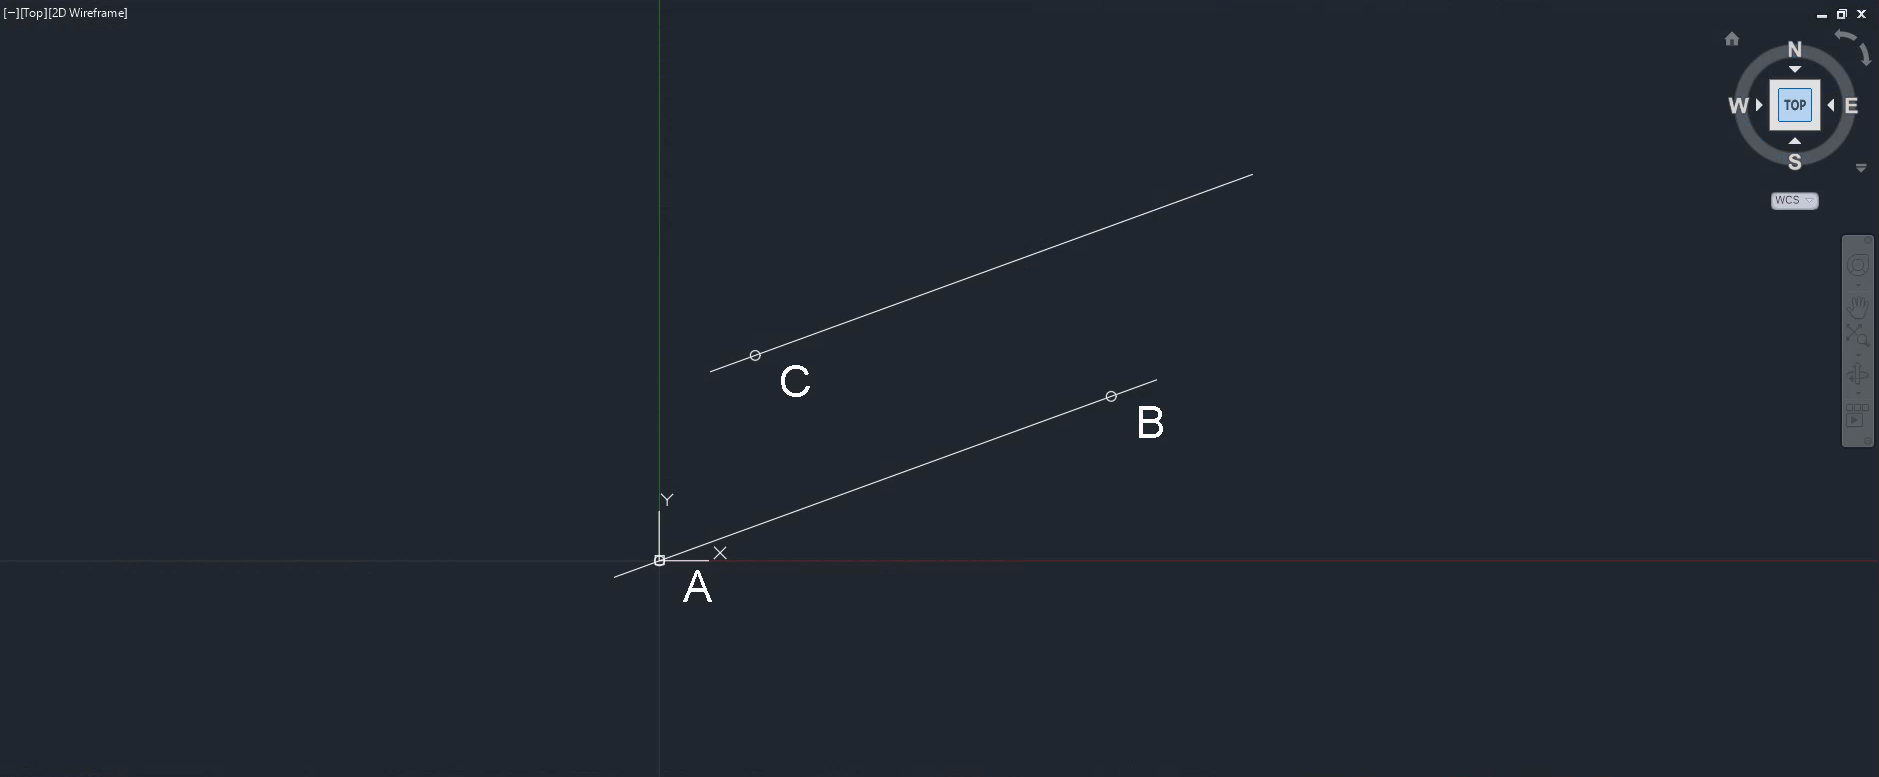
\includegraphics[width=\linewidth]{fig/autocad-parallel} 
  \caption[Parallel lines example using our solution]{
    Parallel lines example from \cref{sec:intro.examples.parallel} revisited
    using our solution's \texttt{parallel} primitive construct.  Output
    visualized in AutoCAD.}%
  \label{fig:solution.impl.gcps.parallel}
\end{figure}

\subsubsection{Circumcenter}%
\label{sec:solution.impl.gcps.circumcenter}

Regarding our circumcenter problem, introduced in
\cref{sec:intro.examples.circumcenter}, we initially solved it by intersecting
two of the three triangle sides' bisectors.  We can still approach the problem
that way, defining a \texttt{circumcenter} function similar to the one in
\cref{lst:solution.impl.gcps.circimpl}.

\begin{listing}[htbp]
  \begin{minted}[linenos=false]{julia}
  circumcenter(a, b, c) = intersection(bisector(a, b), bisector(b, c)) 
  \end{minted}
  \caption[Initial circumcenter solution]{
    Initial implementation of the \texttt{circumcenter} function.}%
  \label{lst:solution.impl.gcps.circimpl}
\end{listing}

However, this is one occasion where this functionality is already present in
\ac{CGAL}.  This is a simple yet perfect demonstration of one of our approach's
benefits with regard to repurposing a comprehensive library with plenty of
functionality, allowing us near-direct reuse without re-implementing it.

\Cref{lst:solution.impl.gcps.circumcenter} illustrates a solution to the
``circumcenter'' problem using \ac{CGAL}'s \texttt{circumcenter} function.  The
program's output can be seen in \cref{fig:solution.impl.gcps.circumcenter}.

\begin{listing}[htbp]
  \inputminted{julia}{jl/ex_circumcenter.jl}
  \caption[Circumcenter example using our solution]{
    Implementation of the circumcenter example illustrated in
    \cref{fig:intro.example.circumcenter} using Khepri alongside our solution.}%
  \label{lst:solution.impl.gcps.circumcenter}
\end{listing}

\begin{figure}[htbp]
  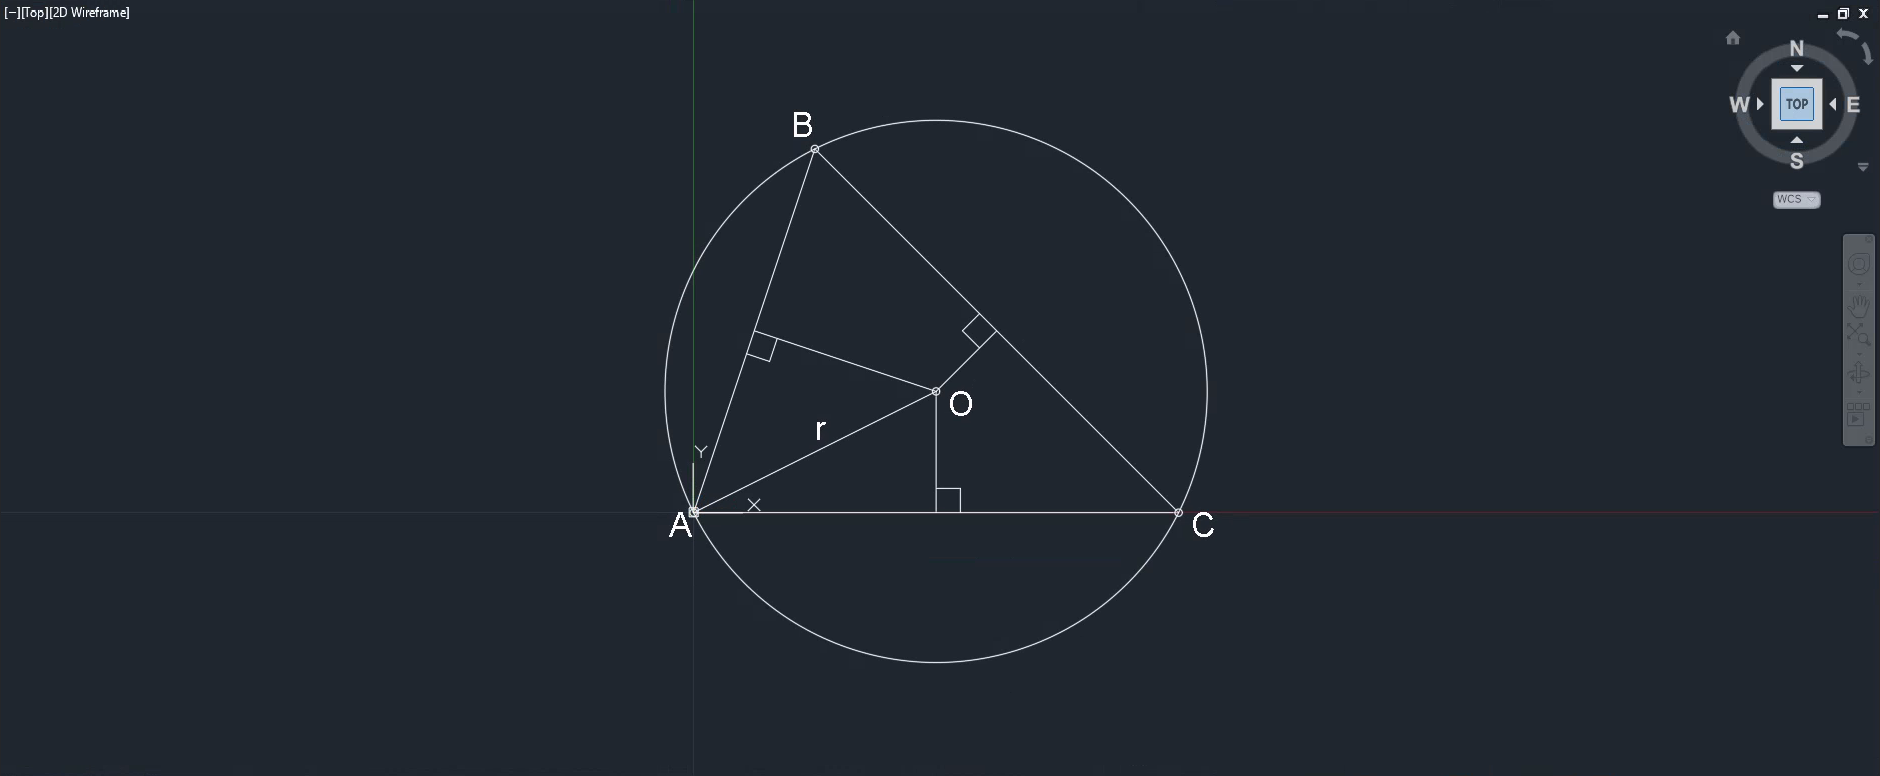
\includegraphics[width=\linewidth]{fig/autocad-circumcenter} 
  \caption[Circumcenter example using our solution]{
    Circumcenter example revisited using our solution's \texttt{circumcenter}
    primitive construct.  Output visualized in AutoCAD.}%
    \label{fig:solution.impl.gcps.circumcenter}
\end{figure}

\subsubsection{Circle tangent to a line}%
\label{sec:solution.impl.gcps.tangcirc2line}

Moving on to a set of problems that cannot as directly be solved by \ac{CGAL} is
that of tangencies.  Generally speaking, there are specific constructs available
in \ac{CGAL} that solve these problems.  However, we can once again repurpose
the ones we have and build on top of them.

This problem involves computing a circle that is tangent to an already existing
line.  Given the circle's center \texttt{o} and the line \texttt{l} we want the
circle to be tangent to, the tangent circle is such that its radius is the
minimal distance between its center point \texttt{o} and the line \texttt{l}.
The implementation of the problem's solution can be seen in
\cref{lst:solution.impl.gcps.tangcircle2line}.

\begin{listing}[htb]
  \begin{minted}[linenos=false]{julia}
  tangent_circle(o::Point2, l::Line2) = Circle2(o, squared_distance(o, l))
  \end{minted}
  \caption[Circle tangent to a line]{
    Implementation of the ``Circle tangent to a line'' problem.}%
  \label{lst:solution.impl.gcps.tangcircle2line}
\end{listing}

Notice this solution considers we are working with infinite lines, not
necessarily line \textit{segments} in general.  Were we to apply the same simple
approach to a line segment, the circle would end up tangent to the line segment
as well.  However, the resulting circle could be tangent to one of the segment's
endpoints instead of tangent to a point along the segment.  In some cases, the
latter behavior may be preferred, for which adjustments to the solution must be
made, such as indicating that there is no solution for the given center point.

We did not implement such a scenario regarding line segments, because much like
the other primitives, it was created to satisfy a specific use case's
requirements.  A potential solution to that specific problem could be obtained
reusing the \texttt{tangent\_circle} function, however.  We would then need to
verify if the circle would fall somewhere between the segment's endpoints.
Otherwise, there would not be a solution available.

\subsubsection{Tangent circles}%
\label{sec:solution.impl.gcps.tangentcircles}

Another instance of tangency is that of two circles tangent to each other.  This
proves to be a relatively more complex problem due to how the circles may be
positioned.

Given two circles \texttt{c\textsubscript{1}} and \texttt{c\textsubscript{2}},
and a vector \texttt{v} used to indicate the point of tangency on
\texttt{c\textsubscript{1}}, we draw a circle centered on said point with the
same radius as \texttt{c\textsubscript{2}} and intersect it with a ray
\texttt{r'} originating from the former circle's center, giving us a point
\texttt{f}.  This ray may be directed in one of two ways, determining if the
resulting circle contains both circles or not.  We then compute the bisector
\texttt{b} between \texttt{f} and \texttt{c\textsubscript{2}}.  We test if we
are in a situation where the resulting circle would instead turn out to be a
line.  If that is the case, we produce an error.  Otherwise, we construct the
tangent circle.

\Cref{lst:solution.impl.gcps.tangentcircles} contains the solution to the
problem, assisted by our own definition of the intersection function between a
circle and a ray, listed in \cref{lst:solution.impl.gcps.circrayint}.

\begin{listing}[htb]
  \inputminted[firstline=11]{julia}{jl/tangent_circles.jl}
  \caption[Tangent circles]{
    Implementation of the ``Tangent circles'' problem.}%
  \label{lst:solution.impl.gcps.tangentcircles}
\end{listing}

\begin{listing}
  \inputminted[lastline=9]{julia}{jl/tangent_circles.jl}
  \caption[Circle-Ray intersection]{
    Implementation of the intersection between a circle and a ray.}%
  \label{lst:solution.impl.gcps.circrayint}
\end{listing}

\subsubsection{Tangent lines between circles}%
\label{sec:solution.impl.gcps.tanglines2circles}

Another problem that surfaced in a case study earlier illustrated in
\cref{fig:intro.chair} is that of computing tangent lines between two circles.
It is a slightly more complex problem for which there is no obvious solution.
Fortunately, a constructive solution to this problem already
exists,\footnote{\url{https://en.wikipedia.org/wiki/Tangent_lines_to_circles\#Synthetic_geometry}}
an approach our implementation is based on.

This problem's complexity lead us to break it into two different problems.
First, we must determine the lines tangent to a circle that pass through a given
point (\cref{lst:solution.impl.gcps.tanglines2circles}).  Then, repurposing the
solution to that problem, we solve the overarching problem of determining the
lines tangent between circles (\cref{lst:solution.impl.gcps.tanglines2circle}).
This is another example of how we can compose a smaller set of primitives to
solve a larger problem.

\begin{listing}[htbp]
  \inputminted[firstline=2,lastline=16]{julia}{jl/circ_tangent_lines.jl}
  \caption[Tangent lines to a circle]{
    Implementation of the ``Tangent lines to a circle'' sub-problem.}%
  \label{lst:solution.impl.gcps.tanglines2circles}
\end{listing}

\begin{listing}[htbp]
  \caption[Tangent lines between circles]{
    Implementation of the ``Tangent lines between circles'' problem by way of
    composition with the solution of ``Tangent lines to a circle''.}%
  \label{lst:solution.impl.gcps.tanglines2circle}
  \inputminted[firstline=18,lastline=59]{julia}{jl/circ_tangent_lines.jl}
\end{listing}

Our implementation returns the results in a deterministic way, facilitating
result choice.  The line segments are oriented from \texttt{c\textsubscript{1}}
to \texttt{c\textsubscript{2}}, with the internal tangents surrounded by the
external tangents, sorted in a counterclockwise orientation.


% !TeX root = ../../main.tex
\section{Trade-offs}%
\label{sec:solution.tradeoffs}

Since virtually nothing comes without trade-offs and compromises, it is
paramount we address our implementation's qualities, both negative and positive.

Relying on a library such as \ac{CGAL} proves to be as great as it can be
daunting.  As mentioned in \cref{sec:solution.impl.cgal}, \ac{CGAL} is a very
comprehensive and mature software library, arguably even far exceeding our
solution's needs, yet fitting it perfectly.

It is, however, an external component, and with every such component, we do not
hold as much control over it as if it was internal instead.  For example, in the
advent a bug is found within \ac{CGAL}, one cannot \emph{immediately} fix it by
altering its source code and use this fixed version.\footnote{Not unless one
wishes to maintain an entirely separate version of the software until this local
fix is applied upstream.  It can be tiresome if we wish to distribute our
solution and have to redistribute a different version of \ac{CGAL} as well
instead of the globally available releases.}  Important emphasis on bugs not
being \emph{immediately} fixable lest we forget \ac{CGAL} is still an
open-source project arguably anyone can contribute to.  Alas, said contribution
deployments are still out of our control.  In hindsight, however, it can be
considered as just an inconvenience since it is a project that is actively
maintained by very knowledgeable people in the computer graphics and mathematics
fields.

\Ac{CGAL} is also a highly generic library, making heavy use of C++ templates.
Although its design makes usage an elegant experience, the same cannot be said
when trying to map its constructs to another language, especially a language
with a different memory management paradigm which could lead to some nasty
low-level ordeals.  Luckily, \texttt{CxxWrap.jl} helps us solve most, if not
all, of those issues.

Regarding our wrapper code, there is one small problem we still technically did
not solve.  We are still mapping \ac{CGAL} types in an opaque fashion, fixing
the kernel on the C++ side.\footnote{There are other projects that attempt to
make \ac{CGAL} available in other language that resort to this same trick. See
\url{https://github.com/scikit-geometry/scikit-geometry} and
\url{https://github.com/CGAL/cgal-swig-bindings}.}  Alternative methods of
supplying a different kernel were explored, including deploying a different
library compiled with a different kernel.  Despite not entirely solving the
problem, it offered the user the choice of using exact constructions.  However,
this alternative became unmaintainable and virtually impossible to successfully
employ.  In part due to Julia's package pre-compilation, it is no longer viable
to use this other library.

Ideally, the geometric objects would be parametric, and the kernel (or kernels)
mapped to Julia as well, but we were met with complications that would make it
unfeasible for us to implement our solution.  As a compromise, \texttt{CGAL.jl}
fixed a kernel that provides exact predicates with inexact constructions,
favoring performance over some robustness loss.  Nonetheless, in practical
terms, it suffices for our case.

As an alternative to wrapping \ac{CGAL}, we could have explored other options in
the still growing Julia ecosystem.  Some work seems
promising,\footnote{\url{https://github.com/JuliaGeometry}} but not only are
some libraries still catching up, it is also highly unlikely they will ever meet
the quality of \ac{CGAL}.

Lastly, some of our \ac{GC} primitives employ some computation that can lead to
robustness loss as well.  Primarily the ones that involve circles, non-linear
geometric objects, typically require the computation of a square root to work
with absolute distances.  We typically avoid those computations, postponing them
as much as possible until they are absolutely necessary.  As an example, in the
``tangent lines to a circle'' implementation in
\cref{lst:solution.impl.gcps.tanglines2circles}, we first compare squared
distances before requiring their absolute value.

Be that as it may, due to having fixed a kernel with inexact constructions for
\ac{CGAL}, we are bound with some robustness loss regardless.  At this point, it
can only be mitigated by also ensuring the quality of the inputs given to our
primitives, and that is reliant on the user.  If the user decides to provide
``garbage'' inputs, they will most likely be met with ``garbage'' outputs, a
concern, however, that falls out of the scope of this work.

